\subsection{Setup}\label{Subsec:setup}
In this experiment we test the reliability of the TET compared to the embedding and a bruteforce methods. 

For our experiments we use the MovieLens dataset provided by grouplens\cite{Grouplensdata}. The data is taken from MovieLens, a movie recommendation website. The dataset we use contains $100000$ movie ratings, given by $943$ users, applied to $1682$ movies. All users have rated at least $20$ movies and each user and movie is represented by an Id. The data was generated between September 19th, 1997 and April 22nd, 1998. For the users no additional information is available, other than what can be inferred from the rating data. For the movies we have additional information such as Movie Title, Release year, and Genres.

\begin{figure}[H]
	\centering
	\begin{adjustbox}{width=0.5\textwidth}
		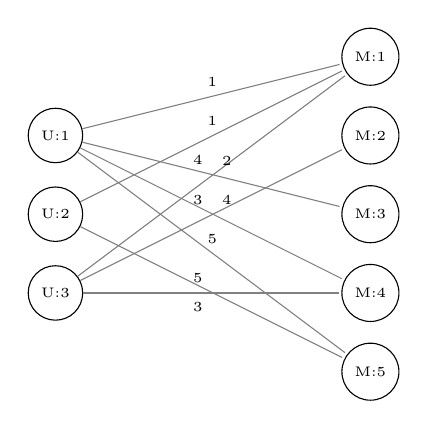
\begin{tikzpicture}[shorten >=1pt, auto, node distance=1cm, ultra thick]
\tikzstyle{node_style} = [circle,draw=black, thin, font=\tiny]
\tikzstyle{edge_style} = [draw=gray, line width=2, thin, font=\tiny ]

\node[node_style] (v1) at (-2,1) {U:1};
\node[node_style] (v2) at (-2,0) {U:2};
\node[node_style] (v3) at (-2,-1) {U:3};

\node[node_style] (v4) at (2,2) {M:1};
\node[node_style] (v5) at (2,1) {M:2};
\node[node_style] (v6) at (2,0) {M:3};
\node[node_style] (v7) at (2,-1) {M:4};
\node[node_style] (v8) at (2,-2) {M:5};
\draw[edge_style]  (v1) edge node[above]{1} (v4);
\draw[edge_style]  (v1) edge node[above left]{4} (v6);
\draw[edge_style]  (v1) edge node[above left]{3} (v7);
\draw[edge_style]  (v1) edge node[above]{5} (v8);
\draw[edge_style]  (v2) edge node[above]{1} (v4);

\draw[edge_style]  (v2) edge node[above left]{5} (v8);
\draw[edge_style]  (v3) edge node[above right]{2} (v4);
\draw[edge_style]  (v3) edge node[above right]{4} (v5);
\draw[edge_style]  (v3) edge node[below left]{3} (v7);
\end{tikzpicture}

	\end{adjustbox}
	\caption{The simple graph}
	\label{fig:graph_representation}
\end{figure}

We create a weighted graph from the data, represented as an edgelist. Each edge is of the form (MovieId, UserId, Rating) where the rating acts as a weight. Each node in the network is either a User or a Movie represented by their Id with the addition of a $U$ on userid and $M$ on movieid respectively, to differentiate them. The movie node will have the additional latent data of genre. A simple example of the graph can be seen in \autoref{fig:graph_representation}.

The data will be split in 10 folds as shown on \autoref{fig:tenfold} using a $80\%/20\%$ split into training- and testset \cite{Ricci2015}. We would like to also add a validation set and the split will therefore be $80\%/10\%/10\%$ or 8 folds/1 fold/1 fold. The splits will be on edge level meaning that training a user will have $80\%$ of their ratings. We will in the validation and test reconstruct or predict the ratings in the set.

\begin{figure}[H]
	\centering
	\begin{adjustbox}{width=0.5\textwidth}
		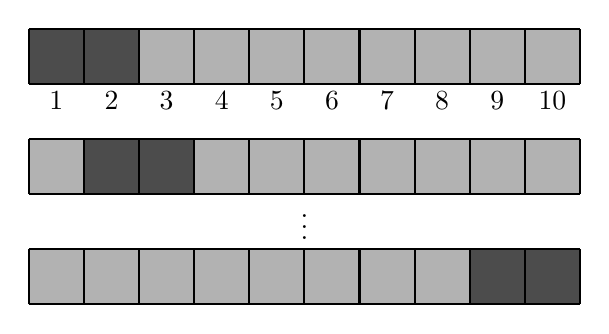
\begin{tikzpicture}[scale=0.7]
\fill[black!70!white] (0,0) rectangle (2,1);
\fill[black!30!white] (2,0) rectangle (10,1);
\draw[step=1cm,black,thick] (0,0) grid (10,1);

\fill[black!70!white] (1,-2) rectangle (3,-1);
\fill[black!30!white] (0,-2) rectangle (1,-1);
\fill[black!30!white] (3,-2) rectangle (10,-1);
\draw[step=1cm,black,thick] (0,-1) grid (10,-2);

\node[thick] at (5,-2.45) {$\vdots$};

\fill[black!70!white] (8,-4) rectangle (10,-3);
\fill[black!30!white] (0,-4) rectangle (8,-3);
\draw[step=1cm,black,thick] (0,-3) grid (10,-4);

\draw (0.5 cm,1pt) node[anchor=north] {$1$};
\draw (1.5 cm,1pt) node[anchor=north] {$2$};
\draw (2.5 cm,1pt) node[anchor=north] {$3$};
\draw (3.5 cm,1pt) node[anchor=north] {$4$};
\draw (4.5 cm,1pt) node[anchor=north] {$5$};
\draw (5.5 cm,1pt) node[anchor=north] {$6$};
\draw (6.5 cm,1pt) node[anchor=north] {$7$};
\draw (7.5 cm,1pt) node[anchor=north] {$8$};
\draw (8.5 cm,1pt) node[anchor=north] {$9$};
\draw (9.5 cm,1pt) node[anchor=north] {$10$};
\end{tikzpicture}
	\end{adjustbox}
	\caption{10 fold example}
	\label{fig:tenfold}
\end{figure}

These split will then be used for building the TETs and embedding nodes.

When these models have been build and trained we will use them to find k-nearest user neighbors according  to each model. With these neighbors we are able to make a prediction on the rating between movies and a user. For the predictions we will use the folded graphs adjacency matrix. We use \autoref{eq:pred} to calculate a predicted rating for the missing ratings in the adjacency matrix.

\begin{equation}\label{eq:pred}
pred(u,m,N) = \overline{r_u}+\sum_{n \in N}w(u,n, N)(r_{n,m}-\overline{r_n})
\end{equation}

\begin{equation}\label{eq:W}
w(u,n, N)=sim(u,n)/\sum_{n' \in N} sim(u,n')
\end{equation}

In \autoref{eq:pred} $u$ and $m$ is the user and movie to calculate a rating between, $N$ is the set of nearest neighbors. $\overline{r_a}$ is the average rating for user $a$ and $r_{b,m}$ is the rating given by user $b$ to movie $m$.
Additionally in \autoref{eq:W} $n$ is a neighboring user to $u$.

The ratings that are missing should be found in the set of the validation fold and test folds.

We will use root mean square error as seen in  \autoref{eq:RMSE}\cite{chai2014root} to find the accuracy of the methods using different folds for test, training and validation set. Where $y \in Y$ is the predicted rating and $x \in X$ is the known rating from the test or validation set.

\begin{equation}\label{eq:RMSE}
RMSE = \sqrt{\frac{1}{n}\sum^n_{i=1}(y_i - x_i)^2}
\end{equation}

A low RMSE is better than a higher RMSE, and a low RMSE is equivalent to a high accuracy.

% There are subtleties that we need to take care of and explain.
	% Do we devide the data on the node level or the edge level?
	% This determines what would we be testing?
	% Lars: i would like to divide on edge level and test on the ability to construct or reconstruct edges between movies and users. We could do the same with list and try to reconstruct the list of bedst movies for a user
% Leave-one-out method
% Splitting the data into folds
	% Lars: i think we should make 20 folds this would allow us to take the standart 70/30 model for splitting training and test and addabt it to a 70/15/15 for training, validation and test.
% Recommender Systems handbook. Read the chapter on evaulating recommender systems.
% Before the experiment: 
	% what is the **Hypothesis**?
	% what is our **Variables**?
	% can the conclutiuon be **Generalized**?
% Offline experiments:
	% what is the **dataset**?
	% what kind of **behavior** does it simulate?
